\documentclass[
	%a4paper, % Use A4 paper size
	letterpaper, % Use US letter paper size
]{jdf}

\usepackage{algorithm}
\usepackage{algpseudocode}
\usepackage{array}
\usepackage{verbatim}
\addbibresource{references.bib}

\author{Mohamed Fayed, Kruthik Ravikanti, Bruce Walker}
\email{mohamed.fayed@gatech.edu, kravikanti3@gatech.edu, bruce.walker@psych.gatech.edu}
\title{Chart-to-Table Conversion: A Survey}

\begin{document}
%\lsstyle

\maketitle

\begin{abstract}
  Multimodal   Large Language Models (MLLMs) have shown impressive visual capabilities in many Visual Question Answering tasks.
    Chart-to-Table Conversion the problem of extracting structured tabular data out of input images, enabling better accessibility and higher storage efficiency.
In this survey, we aim to review the recent advancements in Chart-to-Table task, analyze existing datasets and benchmark some state-of-the-art models on this task.
Our quantitative and qualitative analysis highlights strengths and limitations of those approaches in handling complex charts, preserving numerical precision and generalize across various types of charts.
Our study reveals significant room for improvement in Chart-to-Table Conversion, emphasizing the need for more specialized and robust methods.
   \end{abstract}

   %\tableofcontents

\section{Introduction}\label{sect:intro}
Data visualization is an essential tool for communicating information efficiently, with charts and graphs playing a fundamental role in various domains, including finance, healthcare, and scientific research.
Those visualizations are usually saved in form of images, which are consuming a significant amount of disk storage.
However, extracting structured tabular data from chart images remains a challenging problem, particularly for automated systems.
This challenge is especially critical for accessibility, where individuals with visual impairments rely on machine-readable formats to interpret visual information.

Chart-to-Table is the task of extracting data points from an image of a chart into a table usually in markdown\cite{liu2022deplot,masry2024chartgemma}.
This task was usually tackled via combination of two or more approaches from rule based tecniques, image processing, CNN based deep learning architectures and optical character recognition (OCR).
Those techniques struggle with diverse chart formats, occlusions and variations in visual styles.
More recently, this task was tackled via transformer based models and Multimodal LArge Language Models (MLLMs), which provide more robust solutions.

In this survey, we provide a comprehensive review of Chart-to-Table conversion techniques, covering benchmark datasets, model architectures, evaluation metrics, and existing challenges.
Furthermore, we assess the performance of several state-of-the-art transformers based models, including MLLMs, on this task, highlighting their strengths and weaknesses.
Our findings suggest that while those models exhibit promising results, significant challenges remain, including generalization across different chart types, handling visual input effectively, and improving numerical fidelity.

%\section{Related Work}
% There has been a lot of efforts in summarizing charts, answering questions~\cite{masry2022chartqa,masry2024chartgemma} and converting them into tables~\cite{liu2022deplot}.
% Recently, there has been efforts to analyze the performance of Multimodal Large Language Models (MLLMs) in many all of those tasks.
% In our work, we aim to pay closer attention to Chart-to-Table task.
Our main contributions are:
\begin{enumerate}
     \item Survey recent advancements in Chart-to-Table task, to the best of our knowledge, this is the first survey focusing on Chart-to-Table Conversion,
     \item do comprehensive qualitative and quantitative analysis on various benchmarks covering various common types of charts, and
     %\item Do quantitative analysis for some models on different benchmark datasets,
     %\item Do fine-grained qualitative analysis on various kinds of charts, and
     \item highlight strengths and limitations  of those models, emphasizing on rooms for improvement in tackling Chart-to-Table Conversion.
       \end{enumerate}
\section{Chart-to-Table in Literature}\label{sect:literature}
There has been work in operating in charts in a way or another.
Some researchers aim at converting charts to tables (Chart-to-Table Conversion).
Others have worked on Chart Question Answering and Chart Summarization.
In this work, we focus on Chart-to-Table Conversion.

Chart-to-Table Conversion requires tackling Optical Character Recognition (OCR) and comprehensive Visual Understanding.
In this section, we review related work in Traditional Computer Vision, Deep Learning and Multimodal Large Language Models and how they influenced the evolution of this task.

\subsection{Computer Vision and Deep Learning}\label{ssect:cv-and-dl}
    It all begins with computer vision (CV)-based methods.
    Early attempts to extract tabular data from charts utilized traditional image processing techniques like segmentation and edge detection that could identify visual elements like bars, axes, and legends~\cite{sreevalsan2021tensor}.
    These approaches were effective to some extent, but they struggled with the many variations found in chart styles and occlusions.
    Furthermore, rule-based approaches were often unsuccessful due to complex charts that had overlapping elements or non-standard layouts~\cite{poco2017reverse}.
    As a result, researchers pursued more robust techniques that could better generalize across diverse chart designs.

    Fast forward, researchers gave deep learning a try.
    Systems such as ChartSense~\cite{jung2017chartsense} and ChartOCR~\cite{luo2021chartocr} utilized convolutional neural networks (CNNs) to classify types of charts and extract available data with higher accuracies.
    For instance, ChartOCR combined rule-based methods with deep CNNs to balance generalization and accuracy, achieving strong performance across multiple chart types~\cite{luo2021chartocr}.
    However, these methods needed extensive labeled datasets and lacked generalization across different chart formats.
    %Although CNNs did improve feature extraction, they still struggled with tasks demanding contextual understanding, such as contrasting similar visual elements.
    %To resolve this, researchers started to integrate transformers and multimodal models which allowed for better alignment between textual and visual elements of charts.

    There were many efforts towards handling specific types of charts using either Computer Vision or Deep Learning tecniques.
    ChartParser~\cite{kumar2022chartparser} was a pipeline that focuses on extracting data points for various kinds of bar charts.
    They build rule based algorithm using OCR and image processing techniques.
    Another group of researchers~\cite{li2022chart} focused on extracting underlying data points for camera photos of line charts using custom architecture based on Faster-RCNN~\cite{ren2015faster}.
    They gathered synthetic and real datasets for line charts to improve the performance of their model.
    Their approach shows promising direction in utilizing synthetic data in improving models on real world test images.
    This direction of research highlights challenges of each kind of chart, but it has many disconnected componenets and their results are not necessarily comparable.

    \subsection{Pretraining and Fine-tuning}\label{ssect:pretraining-and-fine-tuning}
After the introduction of transformers~\cite{vaswani2017attention}, Pretraining and Fine-tuning paradigm caught researchers attention.
~\cite{masry2023unichart} gathered a large dataset of 6.9M questions and charts, and used it to pre-train UniChart model.
Another group of researchers~\cite{liu2022matcha} introduced Matcha model, which was a fine-tuned version of Pix2Struct~\cite{lee2023pix2struct} on many tasks including Chart-to-Table.
Later on,~\cite{liu2022deplot} continued pre-training it on Chart-to-Table only to create Deplot.
They forwarded the generated table, human query and an example to FlanPaLM 540B~\cite{chung2024scaling} to answer complex queries.
~\cite{cheng2023chartreader} took a different approach by training a transformers based chart component detection and combine it with extended pretrained T5~\cite{raffel2020exploring} or TaPas~\cite{herzig2020tapas} models.

\subsection{Multimodal Large Language Models (MLLMs)}\label{ssect:mllm}
MLLMs has made significant progress in many tasks and Chart-to-Table was no exception.
One direction is about utilizing general domain LLMs without any tuning.
This direction includes Prompting and Retrieval Augmented Generation techniques~\cite{cao2024graphinsight, voigt2023vist5} to improve the capabilities of general LLMs on chart related tasks.

Another direction is to fine-tune LLMs on Chart-specific Instruction following datasets.
~\cite{masry2024chartinstruct} introduced an instruction following dataset and instruction tuned both LLaMA 2 7B~\cite{touvron2023llama} and Flan-T5 XL 3B~\cite{chung2024scaling} on it.
This instruction tuning strategy was proved to make a generalized model that can handle unseen tasks.
Similarly,~\cite{masry2024chartgemma} fine-tuned PaliGemma~\cite{beyer2024paligemma} to create a 3B ChartGemma.
Another key distinguishing contribution was the method of instruction following data generation.
They generated for predefined tasks, such as Chain of Thought and Chart-to-Tables in form of markdown, and open-ended tasks, such as justifying trends in charts and describing visual elements.

\subsection{Chart-to-Table Evaluation}\label{ssect:task-evaluation}
There has been many metrics for evaluating Chart-to-Table conversion.
In~\cite{luo2021chartocr}, they introduced different metric for each kind of chart:
\begin{enumerate}
         \item For Bar Charts, defined a custom distance function for pairwise point comparison and find minimum cost between prediction and ground truth,
         \item For Line charts, it is handled as continuous similarity problem.œœ
             For each predicted line, it computes the pointwise error between it and each ground truth line, and choose the minimal value.
         \item For Pie Charts, they consider its scoring as sequence matching problem, thus solved using dynamic programming.
              \end{enumerate}
Relative Number Similarity Score~\cite{masry2022chartqa}, also known as Relaxed Accuracy Measure, is about  computing highest accuracy of generated numbers relative to ground truth.
However, it has two main drawbacks:
\begin{enumerate}
         \item It does not consider the position of numbers within the table, and
         \item It ignores textual errors.
              \end{enumerate}
To overcome those limitations, Relative Mapping Similarity (RMS)~\cite{liu2022deplot} computes edit distance between columns names, compute accuracy of values within columns of least edit distances and compute F1-score.
\footnote{our RMS implementation can be found \href{https://github.gatech.edu/mfayed8/GIE-metrics}{here}.}
To learn more about the algorithm, please check appendix~\ref{app:metrics}

\section{Methodology}\label{sect:methodology}
\subsection{Datasets}\label{ssect:datasets}
There has been many datasets introduced for various chart related tasks, with no special attention to Chart-to-Table Conversion.
Aftersome investigation, we found that some datasets include chart images with their corresponding data points.
In our analysis, we focus on reporting scores on two of those testsets: ICPR22~\cite{rousseau2023pattern} and PlotQA~\cite{methani2020plotqa}.

\paragraph{ICPR22 testset~\cite{rousseau2023pattern}} was gathered from research papers published on PubMed Central website.\footnote{\href{https://pmc.ncbi.nlm.nih.gov}{https://pmc.ncbi.nlm.nih.gov}}
Those publications are in biomedical and life sciences domains.
It contains 443 charts splitted into 5 types: Line Charts, Horizontal and Vertical Bar Charts, Scatter Plot and Vertical Box Plot.
It represents a source of real-world generated charts, as they were generated by a large set of researchers.

\paragraph{PlotQA~\cite{methani2020plotqa}} was made by gathering data from various online sources, such as World Bank and Open Data, generate plots out of these data points, and ask annotators questions about those provided charts.
In our work, we focus on the data points used in constructing the charts only.
Its test set contains 33657 charts divided equally among dotted line charts, line charts, and vertical and horizontal bar charts.
We hypothesized that there is no need to test on all $33k$ charts, so we performed comparison among scores for many sample sizes.
Table~\ref{tab:plotqa-scores-for-various-sizes} shows that it is enough to compute scores on a sample of $4k$ randomly selected charts.

\paragraph{Test-Sample:} For the sake of qualitative analysis, we selected a set of charts from PlotQA and ICPR22 testsets.
We randomly selected from each kind of chart in PlotQA.
However, for ICPR22, we selected charts from various data sizes, i.e. of various sizes of json files.
We noticed that larger file sizes are directly correlated to larger count of data points of corresponding charts.
%TODO: add link to download those files.

\subsection{Models}\label{ssect:models}
For our study, we tested the following models in zero-shot setting:
\begin{itemize}
  \item Gemini 1.5 Flash~\cite{team2024gemini}: A general purpose lightweight MLLM, which is larger than other models in this list.
     \item ChartGemma~\cite{masry2024chartgemma}: A specialized model in chart summarization, question answering and reasoning about charts.
       It utilizes PaliGemma 4B~\cite{beyer2024paligemma} as its backbone, and was tuned on Visual Chart Instructions dataset.
     \item Deplot~\cite{liu2022deplot}: A 282M parameters Vision Encoder-Text Decoder transformer architecture.
         It was trained on Chart-to-Table Conversion task.
       \end{itemize}
       \subsection{Prompts}\label{ssect:prompts}
       For deDeplot, we used the prompt recommended in its Hugging Face Model Card: "Generate underlying data table of the figure below:".
       For ChartGemma, we used a simple prompt of "program of thought: extract data points and formulate them into markdown table.
    Note: all data points should be either integer or float.
    Do not write percentages as '56%', but write them as '0.5"

    For Gemini 1.5 Flash, we used a longer prompt, and if its output is not parseable into json object, we prompt it again to fix its format.
    The main prompt is: 
\begin{verbatim}
    "System Message:     You are an EXPERT in scientific visualizations analysis and chart understanding and description.
    You should help people with disabilities in giving an overview of the chart and converting the chart into its original data point form.
        prompt: For the following image, tell me the name of x and y axes, and the values of the each axis.
        The output should be in format of 
        {x_axis_name: x_axis_vavlues_list, y_xis_name: y_axis_values_list}"
        \end{verbatim}

\subsection{Evaluation}\label{ssect:method-eval}
To compare among those models, we compute Relative Mapping Similarity (RMS)~\cite{liu2022deplot} and do qualitative analysis on our Test-Sample testset.

\section{Results and Discussion}\label{sect:results}
\subsection{Scores}\label{ssect:rms}
In this section, we report the scores for each model.
While testing them, we noticed that they have issues in generating markdowns/jsons that can be correctly parsed by pandas.
So, we also report Success Rate (SR) for each model, such that $Success Rate (SR) = count of correctly parsed charts/count of predicted charts within the testset by selected model$.

We reported the results on a subset of PlotQA charts and all of ICPR22.
We were able to generate around 7000 charts from PlotQA.
We hypothesized that the size of 33k test images is very large and we should not find significant difference between scores on 3k and 33k.
To validate this hypothesis, we computed scores for 3k, 4k, 5k and 6k charts to see whether there is a significant need to infere on all 33k images.
Additionally, we computed the scores on the entire testset using deplot model.
As shown in table~\ref{tab:plotqa-scores-for-various-sizes}, there are small differences across samples of 4k, 5k and k relative to variations among scores of all models.
This means that a sample of 4k is sufficient to provide a reliable estimate to model's performance.
\begin{table}
 \begin{tabular}{|c|c|c|}
 Size & ChartGemma & Deplot \\
 \end{tabular}
 \caption{}
 \label{tab:plotqa-scores-for-various-sizes}
  \end{table}


\subsection{Discussion}\label{ssect:discussion}
\begin{table}
 \begin{tabular}{ |c|c|c|c|c|}
 Model & \multicolumn{2}{|c|}{PlotQA} & \multicolumn{2}{|c|}{ICPR22} \\
 & SR & RMS & SR & RMS \\
 Gemini 1.5 Flash & $86.5\%$ & $55.6\%$ & & \\
 ChartGemma & $19.4\%$ & $31.9\%$ & & \\
 Deplot & $33.1\%$ & $51.6\%$ & &  \\
 \end{tabular}
 \caption{Models scores on PlotQA and ICPR22 testsets.}
 \label{tab:final-scores}
  \end{table}

Fianl scores are shown in table~\ref{tab:final-scores}.
Gemini 1.5 Flash achieved the highest Success Rate (SR), indicating its strong ability to produce well-formatted and parseable outputs.
However, Deplot outperformed all models in terms of Relative Mapping Similarity (RMS), showcasing its superior alignment with the ground truth table values.
On the other hand, ChartGemma recorded the lowest performance in both SR and RMS.

The relatively high SR of Gemini 1.5 Flash suggests that a powerful text decoder plays a crucial role in generating structured and clean outputs.
Meanwhile, Deplot’s strong RMS score—despite being a smaller, specialized model—underscores the value of task-specific architectural tuning.
These results suggest that instruction fine-tuning (as in ChartGemma) may not be sufficient to achieve high-quality Chart-to-Table conversions without deeper task alignment and robust visual reasoning.

Low scores of all models in ICPR22 testset suggests that it is difficult testset.
After manual inspection, we noticed that it has many issues causing RMS scores to be low.
One cause is that many line charts have no labels for their lines.
Many columns in tables of the testset contain "unnamed data series 0", which has 1 normalized edit distance with whatever models generate as columns names, thus 0 RMS score occurs frequently.
In a future work, we would also take into account computing RMS both with and without considering normalized edit distance.
Another reason for those low scores is the failure of all models in properly extracting data from scatter plots and vertical box plots, as illustrated in section~\ref{sssect:scatter} and section~\ref{sssect:box} respectively.

\subsection{Text Recognition}\label{ssect:qualitative-text-recognition}
For the sample we analyzed, we found a single error in deplot recognizing name of second row in table 28308 in PlotQA.
Otherwise, all text was correctly recognized by all models.
However, tables~\ref{tab:deplot-plotqa-line-21673}, ~\ref{tab:chartgemma-plotqa-line-21673} and~\ref{tab:gemini-plotqa-line-21673} show models' tendency to labelize even if there are no labels in the input image.
\footnote{the prediction of Gemini and Ground Truth have no labels for x-axis, but ChartGemma made years as labels.}
\footnote{In some cases, the ground truth is mislabelled. The reference has no values for x-axis, but the image includes them as in~\ref{fig:plotqa-line-20049}.}

\subsection{Values Extraction}\label{ssect:values-extraction}
For PlotQA and ICPR22 samples, it is frequent to find errors like:
\begin{enumerate}
     \item rounding errors, e.g. $15.42->15 and 15.6->15$.
     \item Precision Errors: we have noticed that the models can not predict more than 3 digits for Gemini 1.5 Flash and ChartGemma or 4 digits for Deplot per each value, e.g. $126765000.0->156000000$.
     \item In case of near values, e.g. $24.18, 24.09$, there might be some errors, e.g. predicting $23$ instead of $24$.
       For that kind of error, it may result in changing trend, e.g. steady performance may seam as decreasing.
       \footnote{It is worth noting that we have not seen cases where increasing is replaced by decreasing trends or vice versa in our Test-Sample.}
       \item All models can differentiate outputs based on scale, e.g. $156000000 \& 50.2$ for instance.
all models sometimes change scale, e.g. table~\ref{tab:chartgemma-plotqa-line-21673} where ChartGemma returned values multiplied by 10.
However, Deplot is more robust to this error.
       \item Occasionally, ChartGemma and Gemini 1.5 Flash swap two columns as shown in table~\ref{tab:gemini-plotqa-line-18806}.
         As a result, RMS score is significantly lower (f1=$34\%$) than its fixed version (f1=$83\%$).
       \end{enumerate}

       In the following subsubsections, we illustrate issues related to each kind of graphs.

\subsubsection{Bar Charts}\label{sssect:bar-errors}
\begin{enumerate}
    \item All models are good in extracting data points of Horizontal and Vertical bar charts.
        However, Deplot seams better in precision and in extracting negative points as in Figure~\ref{fig:plotqa-vbar-32640}.
       \end{enumerate}
       \begin{figure}
            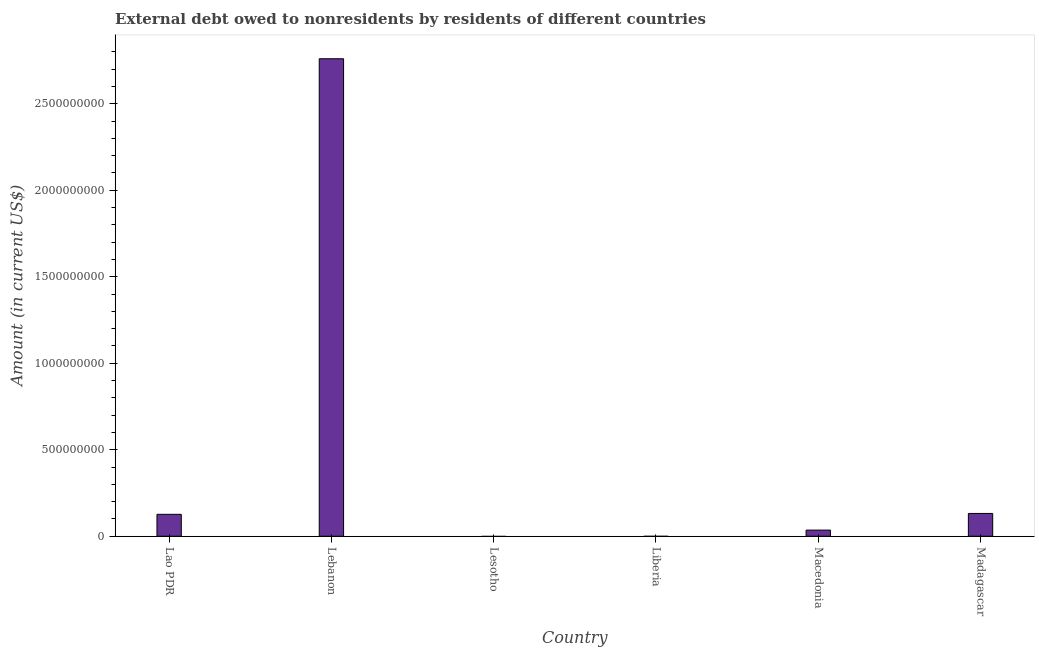
\includegraphics{test-sample/plotqa/images/vertical-bar/32640.png}
            \caption{PlotQA Vertical Bar no. 32640.}
            \label{fig:plotqa-vbar-32640}
             \end{figure}
             \begin{table}
\begin{tabular}{llr}
\toprule
 & Country & Amount (in current US\$) \\
\midrule
0 & Lao PDR & 15000000 \\
1 & Lebanon & 270000000 \\
2 & Lesotho & 0 \\
3 & Liberia & 0 \\
4 & Macedonia & 5000000 \\
5 & Madagascar & 15000000 \\
\bottomrule
\end{tabular}
    \caption{Gemini 1.5 Flash prediction for PlotQA vertical bar \#32640}
    \label{tab:gemini-plotqa-vbar-32640}
\end{table}

             \begin{table}
    \begin{tabular}{lll}
\toprule
 & Country  & Amount (in current US\$)  \\
\midrule
1 & Lao PDR  & 100,000,000  \\
2 & Lebanon  & 270,000,000  \\
3 & Lesotho  & 0  \\
4 & Liberia  & 0  \\
5 & Macedonia  & 30,000,000  \\
6 & Madagascar  & 150,000,000  \\
\bottomrule
\end{tabular}
    \caption{ChartGemma prediction for PlotQA vertical bar \#32640}
    \label{tab:chartgemma-plotqa-vbar-32640}
\end{table}

             \begin{table}
    \begin{tabular}{lr}
Country & Debt \\
Lao PDR & 123191000 \\
Lebanon & 2757587000 \\
Lesotho & -11173000 \\
Liberia & -12609000 \\
Macedonia & 33960000 \\
Madagascar & 130544000 \\
\end{tabular}
    \caption{Deplot prediction for PlotQA vertical bar \#32640}
    \label{tab:deplot-plotqa-vbar-32640}
\end{table}

       \subsubsection{Line Charts}\label{sssect:line-errors}
       \begin{enumerate}
  \item Tables~\ref{tab:deplot-plotqa-line-21673}, ~\ref{tab:chartgemma-plotqa-line-21673} and~\ref{tab:gemini-plotqa-line-21673} show that both models are very good in extracting data points from line charts.
     \item There are some graphs, like~\ref{fig:icpr22-line-6339}, the Gemini API just fails with no clear response message.
       However, it is suspected that the large number of data points might be the reason.
               It is noticable for the same chart to cause Deplot to repeat some rows as shown in table~\ref{tab:deplot-icpr22-line-6339}.
     \item Table~\ref{tab:chartgemma-plotqa-line-20049} shows that ChartGemma may fail in extracting data points from slightly complex graphs.
       It fails in both extracting correct values as well as mapping them to the correct label.
              \end{enumerate}
       Tables~\ref{tab:gemini-plotqa-vbar-25905} and~\ref{tab:chartgemma-plotqa-vbar-25905} include Gemini 1.5 Flash and ChartGemma predictions for figure~\ref{fig:plotqa-vbar-25905} respectively.
\begin{figure}
   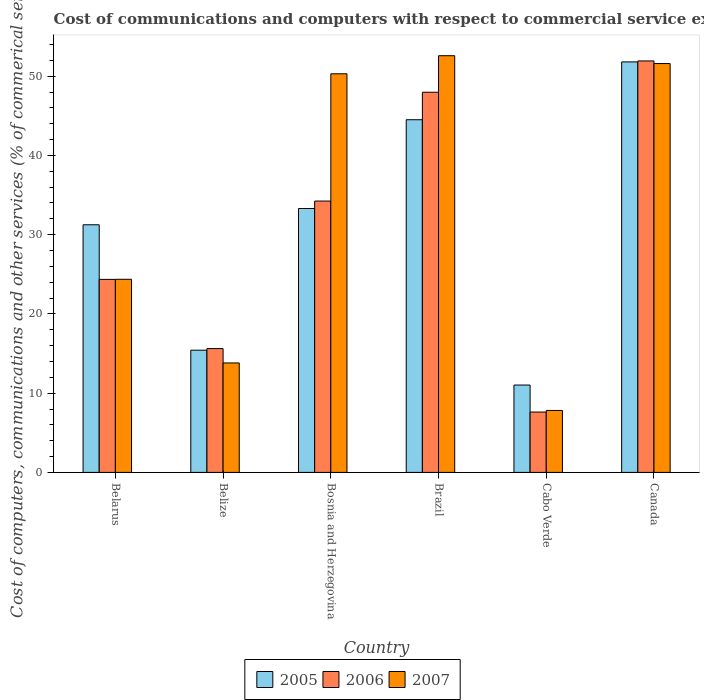
\includegraphics{test-sample/plotqa/images/vertical-bar/25905.png}
   \caption{Vertical Bar Chart example from PlotQA testset.}\label{fig:plotqa-vbar-25905}
   \end{figure}
\begin{table}
    \begin{tabular}{llrrr}
\toprule
 & Country & 2005 & 2006 & 2007 \\
\midrule
0 & Belarus & 31 & 24 & 23 \\
1 & Belize & 15 & 15 & 13 \\
2 & Bosnia and Herzegovina & 33 & 34 & 52 \\
3 & Brazil & 44 & 47 & 52 \\
4 & Cabo Verde & 10 & 7 & 8 \\
5 & Canada & 51 & 52 & 51 \\
\bottomrule
\end{tabular}
    \caption{Gemini 1.5 Flash predictions on Vertical Bar \# 25905}
    \label{tab:gemini-plotqa-vbar-25905}
\end{table}

\begin{table}
\begin{tabular}{lllll}
\toprule
 & Country  & 2005 Cost of computers, communications and other services ($\%$ of commerical service exports)  & 2006 Cost of computers, communications and other services ($\%$ of commerical service exports)  & 2007 Cost of computers, communications and other services ($\%$ of commerical service exports)  \\
\midrule \\
1 & Belarus  & 31  & 24  & 24  \\
2 & Belize  & 15  & 15  & 13  \\
3 & Bosnia and Herzegovina  & 33  & 35  & 49  \\
4 & Brazil  & 45  & 47  & 53  \\
5 & Cabo Verde  & 11  & 8  & 8  \\
6 & Canada  & 52  & 52  & 52  \\
\bottomrule
\end{tabular}
    \caption{ChartGemma predictions for vertical bar image no. 2590 from PlotQA}
    \label{tab:chartgemma-plotqa-vbar-25905}
\end{table}

\begin{table}
    \begin{tabular}{|c|c|c|c|}
Country & 2005 & 2006 & 2007 \\
Belarus & 31.22 & 24.37 & 24.45 \\
Belize & 15.34 & 15.58 & 13.8 \\
Bosnia and Herzegovina & 33.22 & 34.26 & 50.3 \\
Brazil & 44.5 & 47.98 & 52.6 \\
Cabo Verde & 11.06 & 7.63 & 7.76 \\
Canada & 51.81 & 51.93 & 51.6 \\
\end{tabular}
\caption{Deplot predictions on Vertical Bar \# 25905}
    \label{tab:deplot-plotqa-vbar-25905}
\end{table}


\begin{figure}
   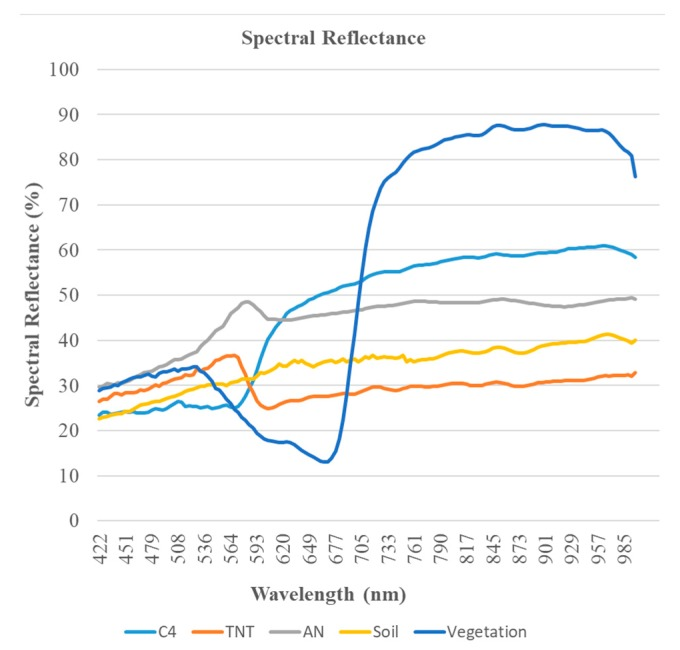
\includegraphics{test-sample/icpr22/images/line/PMC6339093___05.jpg}
   \caption{Example for charts that causes the API to fail.}
   \label{fig:icpr22-line-6339}
   \end{figure}
   \begin{table}
    \begin{tabular}{lllllr}
Wavelength (nm) & C4 & TNT & AN & Soil & Vegetation \\
& 23.7 & 26.8 & 29.6 & 23.7 & 29.4 \\
& 23.9 & 32.6 & 35.6 & 27.9 & 33.8 \\
70.0 & 23.9 & 28.6 & 46.9 & 25.6 & 30.1 \\
50.0 & 25.5 & 33.2 & 36.5 & 29.9 & 33.8 \\
50.0 & 25.2 & 35.6 & 48.3 & 29.5 & 25.2 \\
50.0 & 25.6 & 34.8 & 48.3 & 30.9 & 25.4 \\
50.0 & 25.5 & 34.8 & 48.3 & 30.5 & 25.2 \\
50.0 & 25.8 & 33.8 & 48.3 & 30.5 & 25.2 \\
50.0 & 25.8 & 33.8 & 48.3 & 30.5 & 25.2 \\
50.0 & 25.8 & 33.8 & 48.3 & 30.5 & 25.2 \\
50.0 & 25.8 & 33.8 & 48.3 & 30.5 & 25.2 \\
50.0 & 25.8 & 33.8 & 48.3 & 30.5 & 25.2 \\
50.0 & 25.8 & 33.8 & 48.3 & 30.5 & 25.2 \\
50.0 & 25.8 & 33.8 & 48.3 & 30.5 & 25.2 \\
50.0 & 25.8 & 33.8 & 48.3 & 30.5 & 25.2 \\
50.0 & 25.8 & 33.8 & 48.3 & 30.5 & 25.2 \\
50.0 & 25.8 & 33.8 & 48.3 & 30.5 & 25.2 \\
50.0 & 25.8 & 33.8 & 48.3 & 30.5 & 25.2 \\
50.0 & 25.8 & 33.8 & 48.3 & 30.5 & 25.2 \\
50.0 & 25.8 & 33.8 & 48.3 & 30.5 & 25.2 \\
50.0 & 25.8 & 33.8 & 48.3 & 30.5 & 25.2 \\
50.0 & 25.8 & 33.8 & 48.3 & 30.5 & 25.2 \\
50.0 & 25.8 & 33.8 & 48.3 & 30.5 & 25.2 \\
50.0 & 25.8 & 33.8 & 48.3 & 30.5 & 25.2 \\
50.0 & 25.8 & 33.8 & 48.3 & 30.5 & 25.2 \\
50.0 & 25.8 & 33.8 & 48.3 & 30.5 & 25.2 \\
50.0 & 25.8 & 33.8 & 48.3 & 30.5 & 25.2 \\
50.0 & 25.8 & 33.8 & 48.3 & 30.5 & 25.2 \\
50.0 & 25.8 & 33.8 & 48.3 & 30.5 & 25.2 \\
50.0 & 25.8 & 33.8 & 48.3 & 30.5 & 25.2 \\
\end{tabular}
    \caption{Deplot prediction for ICPR22 line chart \#6339}
    \label{tab:deplot-icpr22-line-6339}
\end{table}

\begin{figure}
   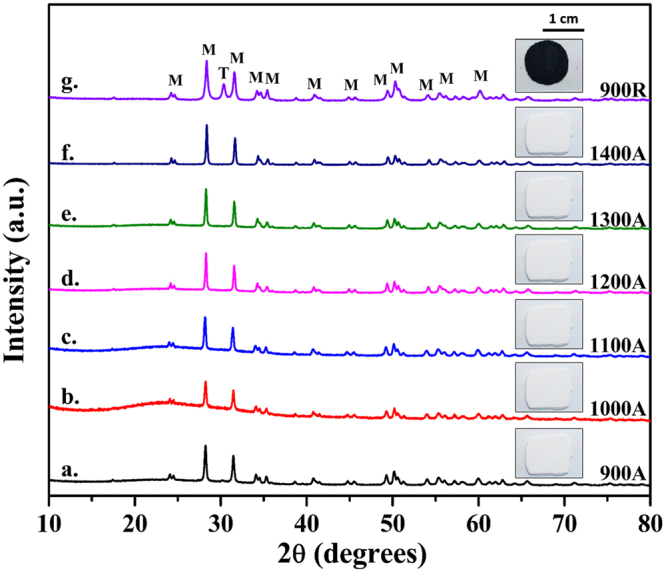
\includegraphics{test-sample/icpr22/images/line/PMC5882956___1_HTML.jpg}
   \caption{A good example for graph in the wild that causes Gemini 1.5 Flash to fail.}
   \label{fig:icpr22-line-5882}
   \end{figure}
\begin{figure}
   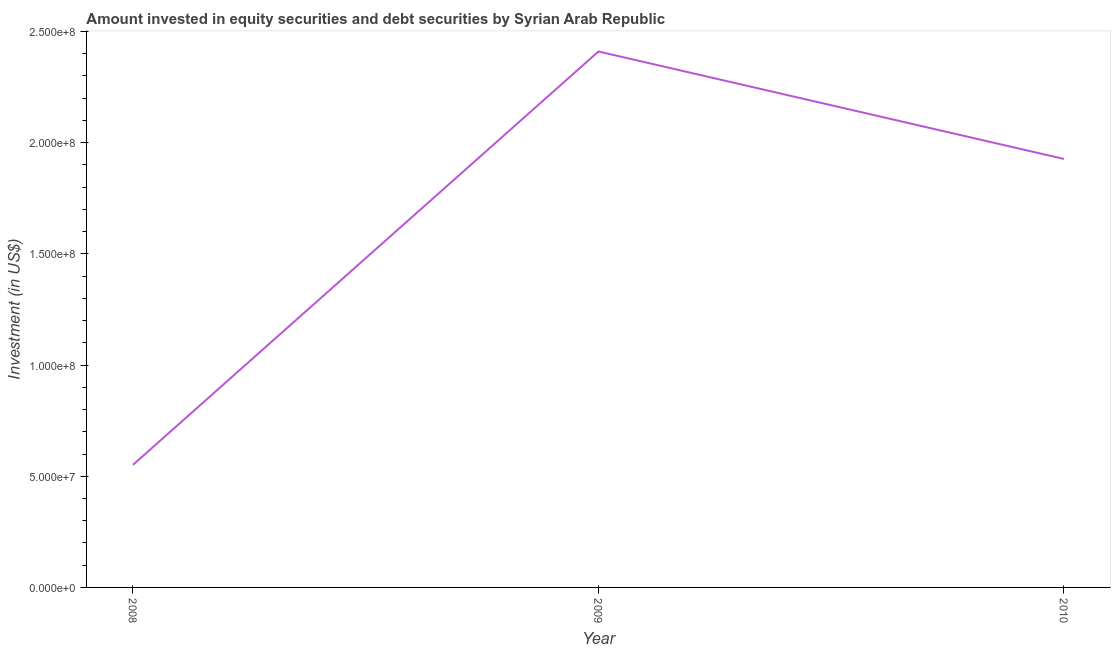
\includegraphics{test-sample/plotqa/images/line/21673.png}
   \caption{Example for Line Chart from PlotQA testset \# 21673 about Portfolio Investment}
   \label{fig:plotqa-line-21673}
   \end{figure}
\begin{table}
\begin{tabular}{lllllll}
\toprule
 & name & color & label & bboxes & y & x \\
\midrule
0 & Portfolio Investment & \#BA55D3 & Portfolio Investment & [{'y': 51, 'x': 132, 'w': 466, 'h': 413}, {'y': 51, 'x': 598, 'w': 465, 'h': 107}] & [55132083.68, 241005430.1, 192682327.3] & [0, 1, 2] \\
\bottomrule
\end{tabular}
     \caption{Reference for Line Chart from PlotQA \#21673 Portfolio Investment}
     \label{tab:plotqa-line-21673-ref}
\end{table}

\begin{table}
    \begin{tabular}{lrr}
\toprule
 & Year & Investment (in USD) \\
\midrule
0 & 2008 & 54000000 \\
1 & 2009 & 240000000 \\
2 & 2010 & 200000000 \\
\bottomrule
\end{tabular}
     \caption{Predicted data points by Gemini 1.5 Flash for Line Chart from PlotQA \#21673 Portfolio Investment}
     \label{tab:plotqa-line-21673-gemini-flash}
     \end{table}

\begin{table}
\begin{tabular}{lll}
\toprule
 & Year  & Investment (in USD)  \\
\midrule
1 & 2008  & 500000000  \\
2 & 2009  & 2400000000  \\
3 & 2010  & 1900000000  \\
\bottomrule
\end{tabular}
    \caption{ChartGemma: prediction for PlotQA line chart \#21673}
    \label{tab:chartgemma-plotqa-line-21673}
\end{table}

\begin{table}
    \begin{tabular}{|c|c|}
Year & Portfolio Investment \\
2008 & 55000000 \\
2009 & 241000000 \\
2010 & 192700000 \\
    \end{tabular}
\caption{Predicted data points by Deplot for Line Chart from PlotQA \#21673 Portfolio Investment}
     \label{tab:deplot-plotqa-line-21673}
\end{table}


\begin{figure}
   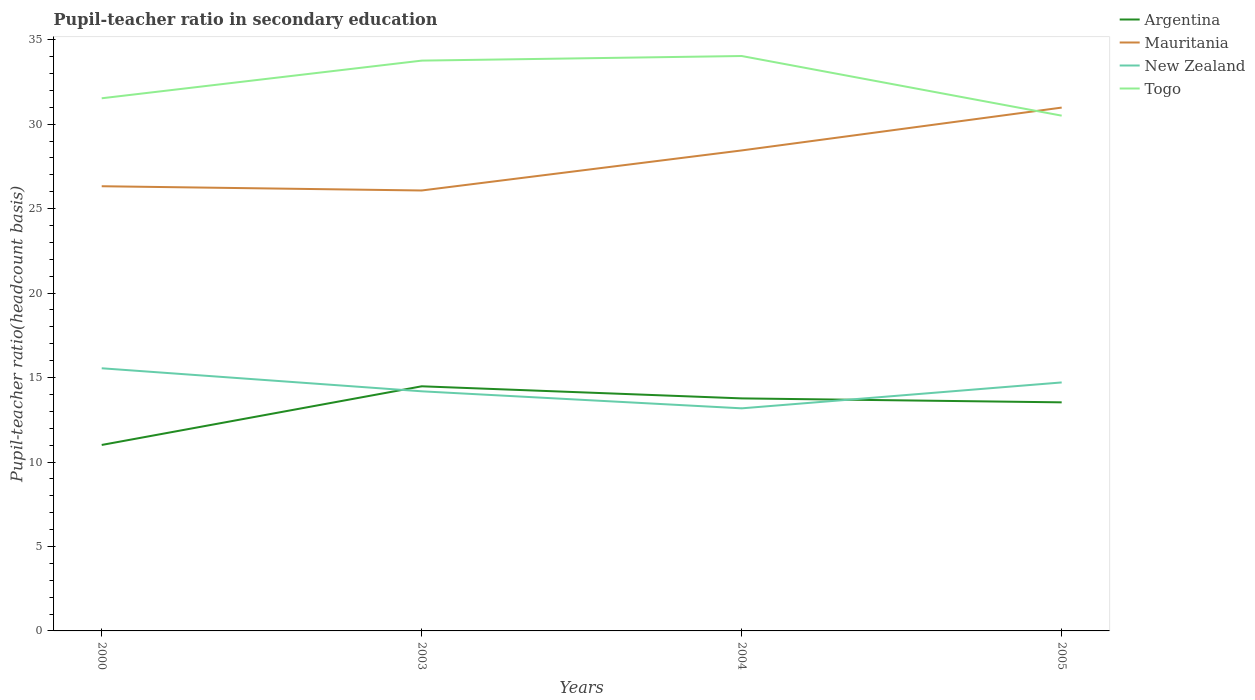
\includegraphics{test-sample/plotqa/images/line/20049-4-lines.png}
   \caption{PlotQA \# 20049: Line chart containing 4 lines.}\label{fig:plotqa-line-20049}
   \end{figure}
   \begin{table}
\begin{tabular}{lllllll}
\toprule
 & name & color & label & bboxes & y & x \\
\midrule
0 & Argentina & \#228B22 & Argentina & [{'y': 386, 'x': 101, 'w': 320, 'h': 58}, {'y': 386, 'x': 421, 'w': 320, 'h': 12}, {'y': 398, 'x': 741, 'w': 320, 'h': 4}] & [11.0102100372314, 14.4826498031616, 13.7663202285767, 13.5325899124146] & [0, 1, 2, 3] \\
1 & Mauritania & \#CD853F & Mauritania & [{'y': 186, 'x': 101, 'w': 320, 'h': 4}, {'y': 150, 'x': 421, 'w': 320, 'h': 40}, {'y': 107, 'x': 741, 'w': 320, 'h': 43}] & [26.3266506195068, 26.0756893157958, 28.4472198486328, 30.9836406707764] & [0, 1, 2, 3] \\
2 & New Zealand & \#66CDAA & New Zealand & [{'y': 368, 'x': 101, 'w': 320, 'h': 23}, {'y': 391, 'x': 421, 'w': 320, 'h': 17}, {'y': 382, 'x': 741, 'w': 320, 'h': 26}] & [15.5497102737427, 14.1861000061035, 13.1779899597168, 14.7109498977661] & [0, 1, 2, 3] \\
3 & Togo & \#90EE90 & Togo & [{'y': 60, 'x': 101, 'w': 320, 'h': 38}, {'y': 56, 'x': 421, 'w': 320, 'h': 4}, {'y': 56, 'x': 741, 'w': 320, 'h': 59}] & [31.5344390869141, 33.7643890380859, 34.03617858886719, 30.5053195953369] & [0, 1, 2, 3] \\
\bottomrule
\end{tabular}
    \caption{Reference table for PlotQA line chart \# 20049}
    \label{tab:ref-plotqa-line-20049}
\end{table}

   \begin{table}
    \begin{tabular}{lrrrrr}
\toprule
 & Year & Argentina & Mauritania & New Zealand & Togo \\
\midrule
0 & 2000 & 10.600000 & 26.000000 & 15.800000 & 31.400000 \\
1 & 2003 & 14.200000 & 25.800000 & 14.000000 & 33.200000 \\
2 & 2004 & 13.600000 & 28.000000 & 13.000000 & 33.800000 \\
3 & 2005 & 13.400000 & 30.200000 & 14.600000 & 30.000000 \\
\bottomrule
\end{tabular}
    \caption{Gemini 1.5 Flash prediction for PlotQA line chart \# 20049}
    \label{tab:gemini-plotqa-line-20049}
\end{table}

   \begin{table}
    \begin{tabular}{llllll}
\toprule
 & Years  & Argentina  & Mauritius  & New Zealand  & Togo  \\
\midrule
1 & 2000  & 21  & 15  & 22  & 11  \\
2 & 2003  & 21  & 14  & 23  & 14  \\
3 & 2004  & 22  & 13  & 23  & 13  \\
4 & 2005  & 21  & 14  & 21  & 14  \\
\bottomrule
\end{tabular}
    \caption{ChartGemma prediction for PlotQA line chart \# 20049. The model fails in mapping lines with values, e.g. Togo column seams more likely to be Argentina. For values, it is obvious that ChartGemma is very far away from correctly detecting values greater than 20!}
    \label{tab:chartgemma-plotqa-line-20049}
\end{table}


\begin{table}
\begin{tabular}{llll}
\toprule
 & Australia & Turkmenistan & United States \\
\midrule
0 & {'Year': 2009.0, 'Subscribers per 100 People': 47.0} & {'Year': 2009.0, 'Subscribers per 100 People': 48.5} & {'Year': 2009.0, 'Subscribers per 100 People': 9.0} \\
1 & {'Year': 2010.0, 'Subscribers per 100 People': 46.0} & {'Year': 2010.0, 'Subscribers per 100 People': 47.5} & {'Year': 2010.0, 'Subscribers per 100 People': 10.0} \\
2 & {'Year': 2011.0, 'Subscribers per 100 People': 45.0} & {'Year': 2011.0, 'Subscribers per 100 People': 46.0} & {'Year': 2011.0, 'Subscribers per 100 People': 11.0} \\
3 & {'Year': 2012.0, 'Subscribers per 100 People': 44.5} & {'Year': 2012.0, 'Subscribers per 100 People': 45.0} & {'Year': 2012.0, 'Subscribers per 100 People': 11.5} \\
4 & {'Year': 2013.0, 'Subscribers per 100 People': 44.0} & {'Year': 2013.0, 'Subscribers per 100 People': 44.0} & {'Year': 2013.0, 'Subscribers per 100 People': 12.0} \\
\bottomrule
\end{tabular}
\caption{Example for Gemini Flash predictions where it swapped the values of Turkmenistan and United States. The swapped table has score of $F1=0.34$ and the corrected version has $F1=0.83$.}
\label{tab:gemini-plotqa-line-18806}
\end{table}

\subsubsection{Scatter Plots}\label{sssect:scatter}
\begin{enumerate}
         \item There is no model capable of handling scatter plots correctly!
          \end{enumerate}
          \begin{figure}
               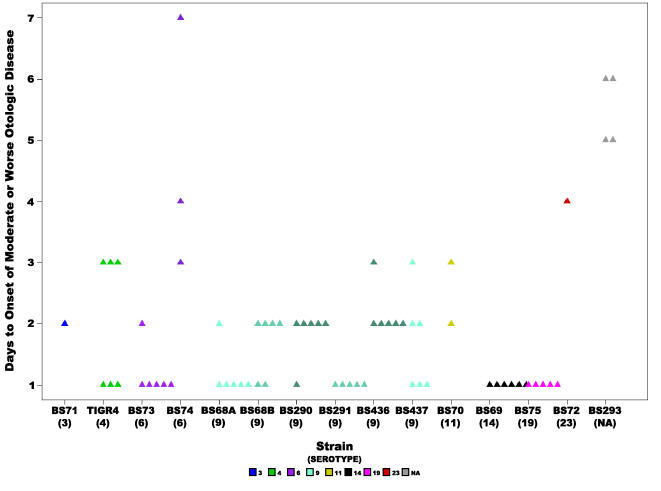
\includegraphics{test-sample/icpr22/images/scatter/PMC2279396___g002.jpg}
               \caption{Scatter Plot from ICPR22 testset \#2279}
               \label{fig:icpr22-scatter-2279}
                \end{figure}
\begin{verbatim}
Ground Truth csv:
\begin{verbatim}
x,y
BS71\n (3),1.9980978260869584
\end{verbatim}

Deplot output csv:
\begin{verbatim}
X,Y,Label
2,1,"1 
 8871
(3)"
2,1,"3 
 8874
(4)"
3,1,"2 
 8873
(6)"
2,1,"1 
 8874
(6)"
2,1,"1 
 8868
(9)"
2,1,"1 
 8868
(9)"
2,1,"1 
 88290
(9)"
2,1,"1 
 88291
(9)"
2,1,"1 
 88434
(9)"
2,1,"1 
 88437
(9)"
2,1,"1 
 8870
(11)"
2,1,"1 
 8860
(14)"
1,1,"1 
 8875
(19)"
1,1,"1 
 8872
(23)"
1,1,"1 
 88293
(NA)"
5,1,1
\end{verbatim}

Gemini 1.5 Flash output json:
\begin{verbatim}
[{"Strain": "BS71", "Serotype": 3, "Days to Onset": 2, "Color": "Blue"}, {"Strain": "TIG4", "Serotype": 4, "Days to Onset": 1, "Color": "Green"}, {"Strain": "TIG4", "Serotype": 4, "Days to Onset": 3, "Color": "Green"}, {"Strain": "BS73", "Serotype": 6, "Days to Onset": 1, "Color": "Purple"}, {"Strain": "BS73", "Serotype": 6, "Days to Onset": 2, "Color": "Purple"}, {"Strain": "BS74", "Serotype": 6, "Days to Onset": 1, "Color": "Purple"}, {"Strain": "BS74", "Serotype": 6, "Days to Onset": 4, "Color": "Purple"}, {"Strain": "BS68A", "Serotype": 9, "Days to Onset": 1, "Color": "Aqua"}, {"Strain": "BS68A", "Serotype": 9, "Days to Onset": 2, "Color": "Aqua"}, {"Strain": "BS68B", "Serotype": 9, "Days to Onset": 1, "Color": "Aqua"}, {"Strain": "BS68B", "Serotype": 9, "Days to Onset": 2, "Color": "Aqua"}, {"Strain": "BS290", "Serotype": 9, "Days to Onset": 1, "Color": "Aqua"}, {"Strain": "BS290", "Serotype": 9, "Days to Onset": 2, "Color": "Aqua"}, {"Strain": "BS290", "Serotype": 9, "Days to Onset": 3, "Color": "Gray"}, {"Strain": "BS291", "Serotype": 9, "Days to Onset": 1, "Color": "Aqua"}, {"Strain": "BS291", "Serotype": 9, "Days to Onset": 2, "Color": "Aqua"}, {"Strain": "BS291", "Serotype": 9, "Days to Onset": 3, "Color": "Gray"}, {"Strain": "BS436", "Serotype": 9, "Days to Onset": 1, "Color": "Aqua"}, {"Strain": "BS436", "Serotype": 9, "Days to Onset": 2, "Color": "Aqua"}, {"Strain": "BS436", "Serotype": 9, "Days to Onset": 3, "Color": "Gray"}, {"Strain": "BS437", "Serotype": 11, "Days to Onset": 1, "Color": "Aqua"}, {"Strain": "BS437", "Serotype": 11, "Days to Onset": 2, "Color": "Aqua"}, {"Strain": "BS437", "Serotype": 11, "Days to Onset": 3, "Color": "Green"}, {"Strain": "BS70", "Serotype": 11, "Days to Onset": 3, "Color": "Yellow"}, {"Strain": "BS69", "Serotype": 14, "Days to Onset": 1, "Color": "Black"}, {"Strain": "BS69", "Serotype": 14, "Days to Onset": 1, "Color": "Black"}, {"Strain": "BS75", "Serotype": 19, "Days to Onset": 1, "Color": "Purple"}, {"Strain": "BS75", "Serotype": 19, "Days to Onset": 1, "Color": "Purple"}, {"Strain": "BS72", "Serotype": 23, "Days to Onset": 1, "Color": "Purple"}, {"Strain": "BS72", "Serotype": 23, "Days to Onset": 4, "Color": "Red"}, {"Strain": "BS293", "Serotype": "NA", "Days to Onset": 5, "Color": "Gray"}, {"Strain": "BS293", "Serotype": "NA", "Days to Onset": 6, "Color": "Gray"}]
\end{verbatim}

ChartGemma output text:
\begin{verbatim}
The table should have two columns: 'Strain' and 'Days to Osse'. Each row in the table should correspond to a strain and its associated 'Days to Osse' value.
\end{verbatim}

\end{verbatim}
\subsubsection{Box Plots}\label{sssect:box}
\begin{enumerate}
         \item Gemini 1.5 Flash was the only model to correctly extract data points from vertical box plots.
             However, comparing Gemini 1.5 Flash's output to ground truth table needs custom logic because some graphs have more than one data series.
              \end{enumerate}
              \begin{figure}
                   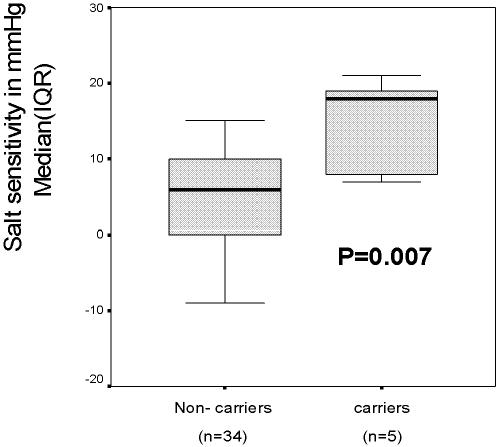
\includegraphics{test-sample/icpr22/images/vertical-box/PMC1855992___g001.jpg}
                   \caption{Vertical Box Plot from ICPR22 testset \#1855}
                   \label{fig:icpr22-box-185}
                    \end{figure}
               \begin{verbatim}
               Ground Truth csv:
               \begin{verbatim}
series_name,subplot_name,first_quartile,max,median,min,third_quartile
[unnamed data series #0],Non - carriers,0.11198945981554975,15.131752305665346,5.9617918313570515,-8.847167325428195,9.914361001317525
[unnamed data series #0],carriers,7.964426877470356,21.034255599472985,17.87220026350461,6.963109354413704,18.873517786561266
\end{verbatim}

               Deplot prediction:
               \begin{verbatim}
Metric,Group,Value
"Salt sensitivity in mm<0xE2><0x80><0xA0>
Median(IQR) 
 Non- carriers
(n=34)",carriers (n=5),10.0
"Salt sensitivity in mm<0xE2><0x80><0xA0>
Median(IQR) 
 Non- carriers
(n=34)",Group1,21.0
\end{verbatim}

               Gemini 1.5 Flash prediction:
               \begin{verbatim}
series_name,subplot_name,first_quartile,max,median,min,third_quartile
[unnamed data series #0],Non - carriers,0.11198945981554975,15.131752305665346,5.9617918313570515,-8.847167325428195,9.914361001317525
[unnamed data series #0],carriers,7.964426877470356,21.034255599472985,17.87220026350461,6.963109354413704,18.873517786561266
\end{verbatim}

               ChartGemma's  output markdown:
               \begin{verbatim}
The table should have two columns: 'Non-carriers' and 'Carriers'. Each row in the table should correspond to a group: 'Non-carriers' has 34 individuals and 'Carriers' has 5 individuals.
\end{verbatim}

               \end{verbatim}

\section{Conclusion and Recommendations}\label{sect:conclusion}
In conclusion, our study provides a comprehensive evaluation of the performance of various models on chart-to-table Conversion.
Our results show that while some models excel in certain types of charts, none of them perform evenly across all chart types.
This highlights the complexity and diversity of chart-to-table tasks, which require specialized models or very capable large general models.

Our findings have important implications for researchers and practitioners working on data extraction and analysis.
They suggest that future research should focus on developing more robust and flexible models that can handle a wide range  of chart types and styles.
Additionally, our results emphasize the need for larger and more diverse datasets to train and evaluate these models.

Overall, our study contributes to a deeper understanding of the challenges and opportunities in chart-to-table tasks and provides a foundation for future research in this area. 
We hope that our findings will fosters further innovation and improvement in data extraction and analysis.

\section{Limitations}\label{sect:limitations}
One limitation of our analysis is testing pre-trained models exclusively and did not test models like ChartOCR.
All those models are not directly comparable and have no existing weights and implementation to easily test.
This has been left for future work.

\section{Acknowledgments}
This research was supported in part through research cyberinfrastructure resources and services provided by the Partnership for an Advanced Computing Environment (PACE)~\cite{pace2017partnership} at the Georgia Institute of Technology, Atlanta, Georgia, USA.

\section{References}
\printbibliography[heading=none]

\appendix
\section{Evaluation Metrics}\label{app:metrics}
\subsection{Relative Mapping Similarity (RMS)}\label{app:rms-algorithm}
\begin{algorithm}
    \begin{algorithmic}[1]
 \Require $prp$ (Predicted Table), $t$ (Ground Truth Table)
        \Ensure $rms\_precision, rms\_recall, rms\_f1$

        Compute Normalized Edit Distance between $p_r || p_c$ and $t_r || t_c$
    , where $||$ is concatenation operator.
        Compute pairwise similarities matrix
        make binarized similarities matrix by inserting 1 in place of highest similarities and zeros otherwise.
        \For $p_i$ in p.values:
        \For $t_j$ in t.values:
        $d_{theta_{ij}} = min(1, \frac{|p_i - t_j|}{|t_j|})$
        $d_{tao_{theta_{ij}}} = (1-Normalized Edit Distance) * (1-d_{theta})$
        \EndFor
        \EndFor
        $RMS_{precision} = \sum_{i} \sum_j d_{tao_{theta_{ij}}} / len(p)$
        $RMS_{recall} = \sum_{i} \sum_j d_{tao_{theta_{ij}}} / len(t)$
        $RMS_{f1} = 2 * \frac{RMS_{precision} * RMS_{recall}}{RMS_{precision} + RMS_{recall}}$
    \end{algorithmic}
\end{algorithm}
% \subsection{ChartOCR Bar Chart Metric}
% \subsection{ChartOCR Line Chart Metric}
% \subsection{ChartOCR Pie Chart Metric}
\subsection{metrics introduced in ChartOCR}\label{ssect:chartocr-metrics}
In this subsection, we illustrate metrics introduced by~\cite{luo2021chartocr}.
\subsubsection{Bar Chart Metric}

Given a predicted bounding box $p = [x_p, y_p, w_p, h_p]$ and a ground truth box $g = [x_g, y_g, w_g, h_g]$, the distance function $D(p, g)$ is defined as:

\[
D(p, g) = \min\left(1, \left\lvert \frac{x_p - x_g}{w_g} \right\rvert + \left\lvert \frac{y_p - y_g}{h_g} \right\rvert + \left\lvert \frac{h_p - h_g}{h_g} \right\rvert\right)
\]

Width $w$ is ignored because it does not affect chart reading.

Construct a pairwise cost matrix $C$ between predicted and ground truth boxes, then solve a minimum cost assignment problem using the Hungarian algorithm. The final score is:

\[
\text{Score} = 1 - \frac{\text{min cost}}{K}, \quad \text{where } K = \max(N, M)
\]

Here $N$ and $M$ are the number of predicted and ground truth boxes respectively.

\subsubsection{Line Chart Metric}

Let $P = \{(x_1, y_1), \ldots, (x_N, y_N)\}$ be the predicted points and $G = \{(u_1, v_1), \ldots, (u_M, v_M)\}$ be the ground truth. The recall is defined as:

\[
\text{Rec}(P, G) = \frac{1}{u_M - u_1} \sum_{i=1}^{M} \left(1 - \text{Err}(v_i, u_i, P)\right) \cdot \text{Intv}(i, G)
\]

Where:

\[
\text{Err}(v_i, u_i, P) = \min\left(1, \left\lvert \frac{v_i - I(P, u_i)}{v_i} \right\rvert\right)
\]

$I(P, u_i)$ is the interpolated value of $P$ at $x = u_i$. $\text{Intv}(i, G)$ is the interval weight:

\[
\text{Intv}(i, G) =
\begin{cases}
\frac{u_{i+1} - u_i}{2} & \text{if } i = 1 \\
\frac{u_i - u_{i-1}}{2} & \text{if } i = M \\
\frac{u_{i+1} - u_{i-1}}{2} & \text{otherwise}
\end{cases}
\]

Precision is defined similarly. The final score is the F1-score:

\[
F1 = \frac{2 \cdot \text{Prec} \cdot \text{Rec}}{\text{Prec} + \text{Rec}}
\]

\subsubsection{Pie Chart Metric}

Let $P = [x_1, \dots, x_N]$ and $G = [y_1, \dots, y_M]$ be the predicted and ground-truth value sequences in clockwise order. The match score is computed via dynamic programming:

\[
\text{score}(i,j) = \max\left(
\text{score}(i{-}1, j),
\text{score}(i, j{-}1),
\text{score}(i{-}1, j{-}1) + 1 - \left\lvert \frac{x_i - y_j}{y_j} \right\rvert
\right)
\]

with $\text{score}(0, j) = \text{score}(i, 0) = 0$ for all $i, j$. The final normalized matching score is:

\[
\text{Score} = \frac{\text{score}(N, M)}{M}
\]


\end{document}
